\Appendix{Lampiran 1. Tren Total Emisi GRK Indonesia}
\label{lampiran}

Data yang diambil dari \textit{World Development Indicators} oleh World Bank \cite{worldbank_2023}, menunjukkan \textit{total greenhouse gas emissions (kt of CO2 equivalent)} di Indonesia tahun 2010-2019. Mengindikasikan bahwa tren dari emisi yang ditimbulkan oleh GRK di Indonesia semakin meningkat secara signifikan, pada tahun 2019 dihasilkan sebesar 1.002.369,0 kt of CO2.
\begin{figure}[H]
    \centering
    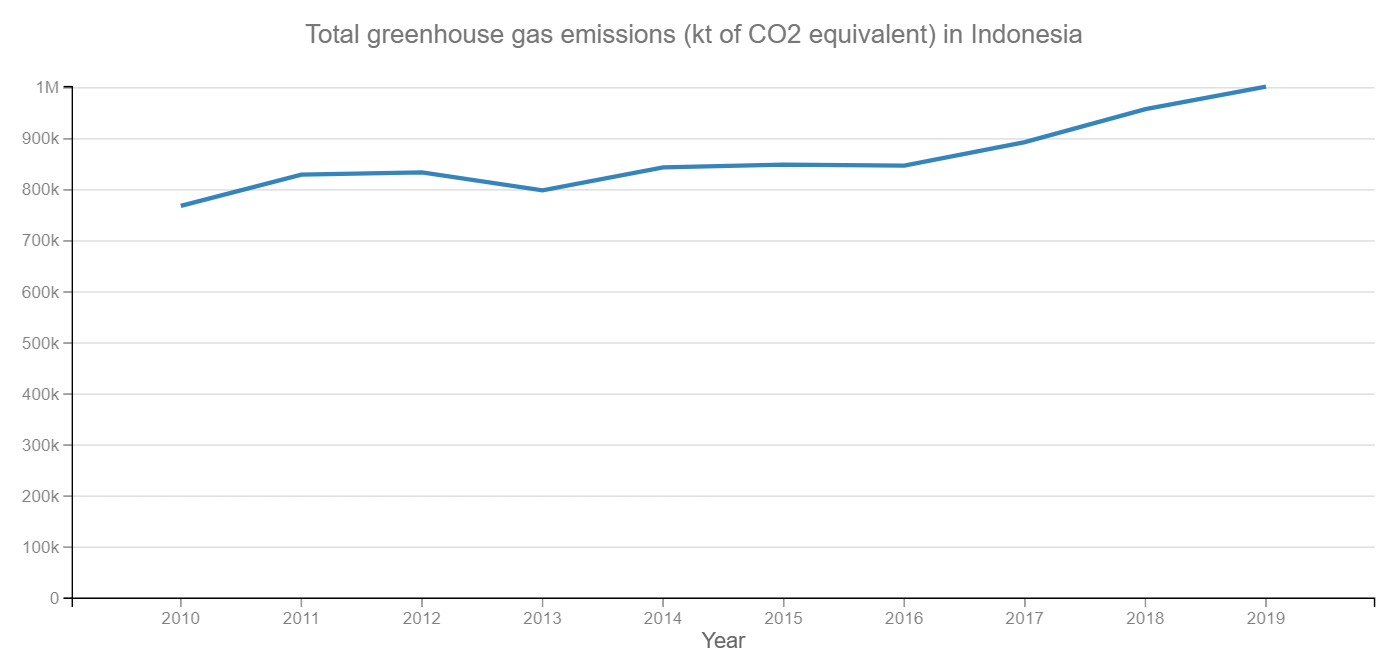
\includegraphics[width=0.9\linewidth]{img/L1.png}
    \caption{Total emisi GRK di Indonesia 2010-2019}
    \label{fig:L1}
\end{figure}
